\chapter{测试与使用}
本设计通过python实现,具有一定的跨平台的能力,在本次测试中,我们对三种主流的系统进行测试,分别是客户端模式和服务端模式的使用。不同系统的环境和配置条件不相同,但是在一定角度上是一致的,这里给出大致的测试步骤:
\begin{itemize}
	\item 配置python环境
	\item 打开宿主主机防火墙
	\item 启动攻击主机服务端,设定服务端IP地址和监听端口
	\item 启动宿主主机客户端,设置IP地址和访问端口
	\item 查看攻击主机是否反弹到shell并确定受控主机身份
\end{itemize}

\section{Mac OS环境下测试}
Mac OS继承于freeBSD,属于类Unix系统,系统默认安装了python环境,因此在测试Mac OS时,我们先检测是否存在python环境,再通过图形界面打开系统的防火墙,启动后门木马程序后执行终端命令完成测试。
\begin{itemize}
	\item 宿主主机:Mac OS Mojave 10.14.3
	\item 攻击主机:Kali Linux 2.0
\end{itemize}






打开终端输入python,先对Mac OS的python环境确认,如果已有python环境,则会显示版本信息同时进入脚本执行界面,如果没有该环境则会提示command not found。
\begin{figure}[h]
\centering
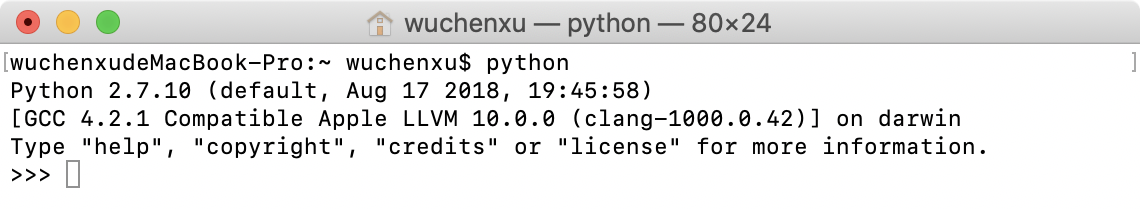
\includegraphics[scale=0.7]{macos环境确认}
\caption{python环境确认}
\label{fig:1}
\end{figure}



之后我们进入系统防火墙。先进入设置,选中安全性与隐私,输入密码,点击铁锁解锁后,这可以点击选中开启宿主主机防火墙。
\begin{figure}[!h]
\centering
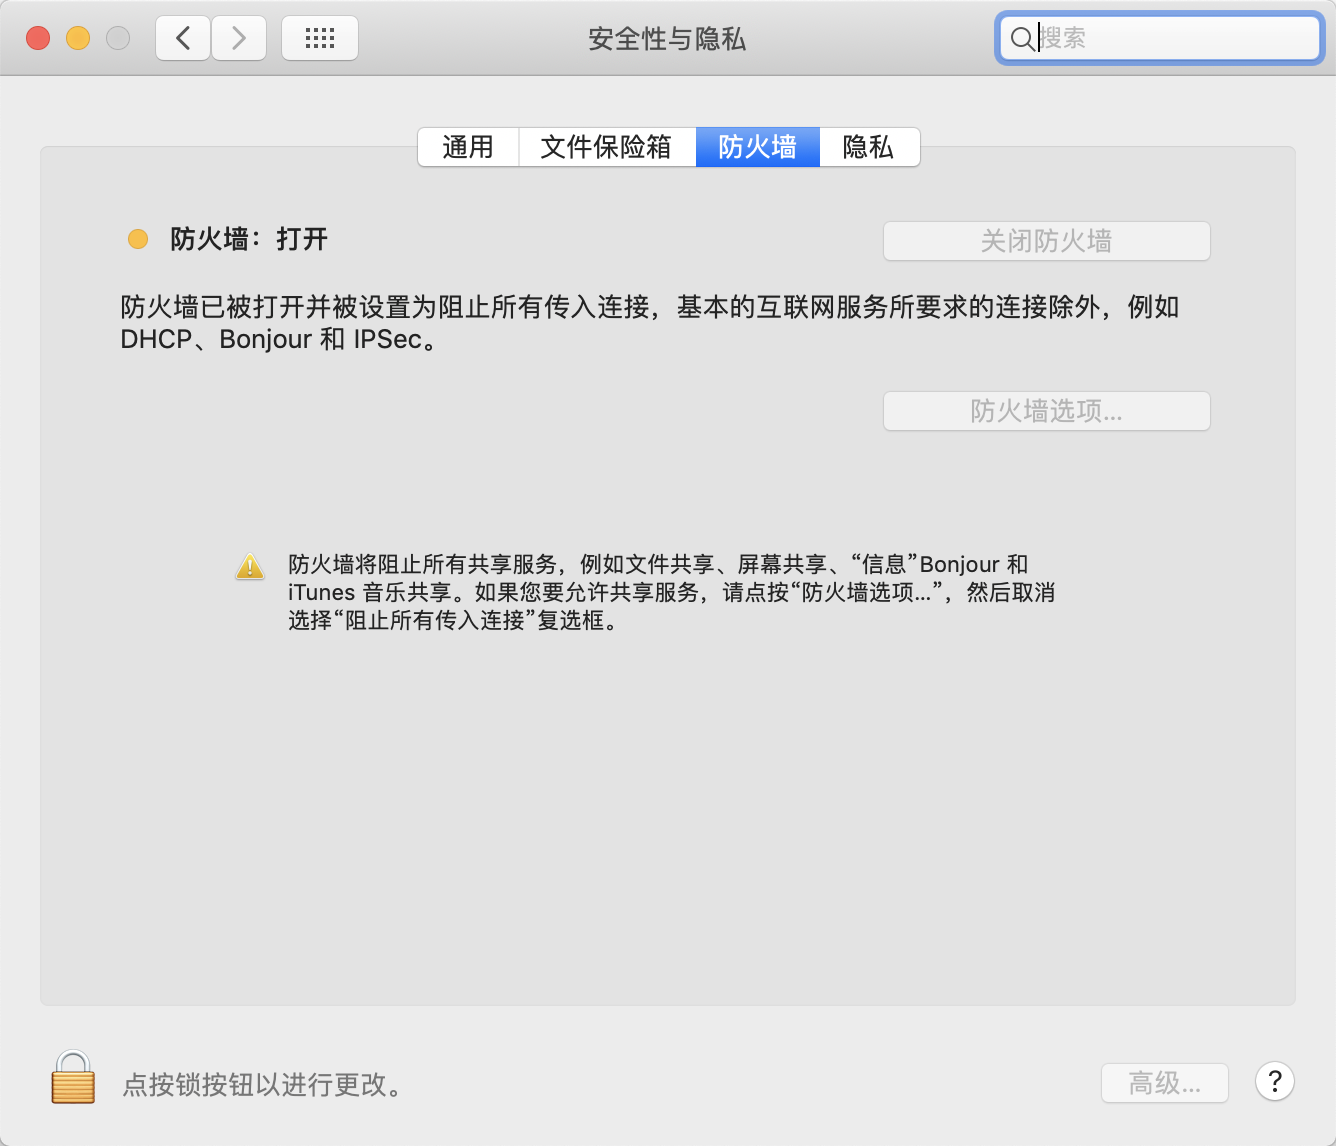
\includegraphics[scale=0.3]{macos防火墙打开}
\caption{Mac OS 防火墙打开}
\label{fig:2}
\end{figure}


Kali Linux 2.0中在终端里通过切换命令跳转到木马程序当前路径下,或者在图形界面在木马程序文件夹内上右击,然后选中在当前文件夹下以终端形式打开,再通过输入python TDshell.py -l [ip] [port]命令来启动攻击机主机服务端的监听功能,设定服务端IP地址和监听端口。
\begin{figure}[h]
\centering
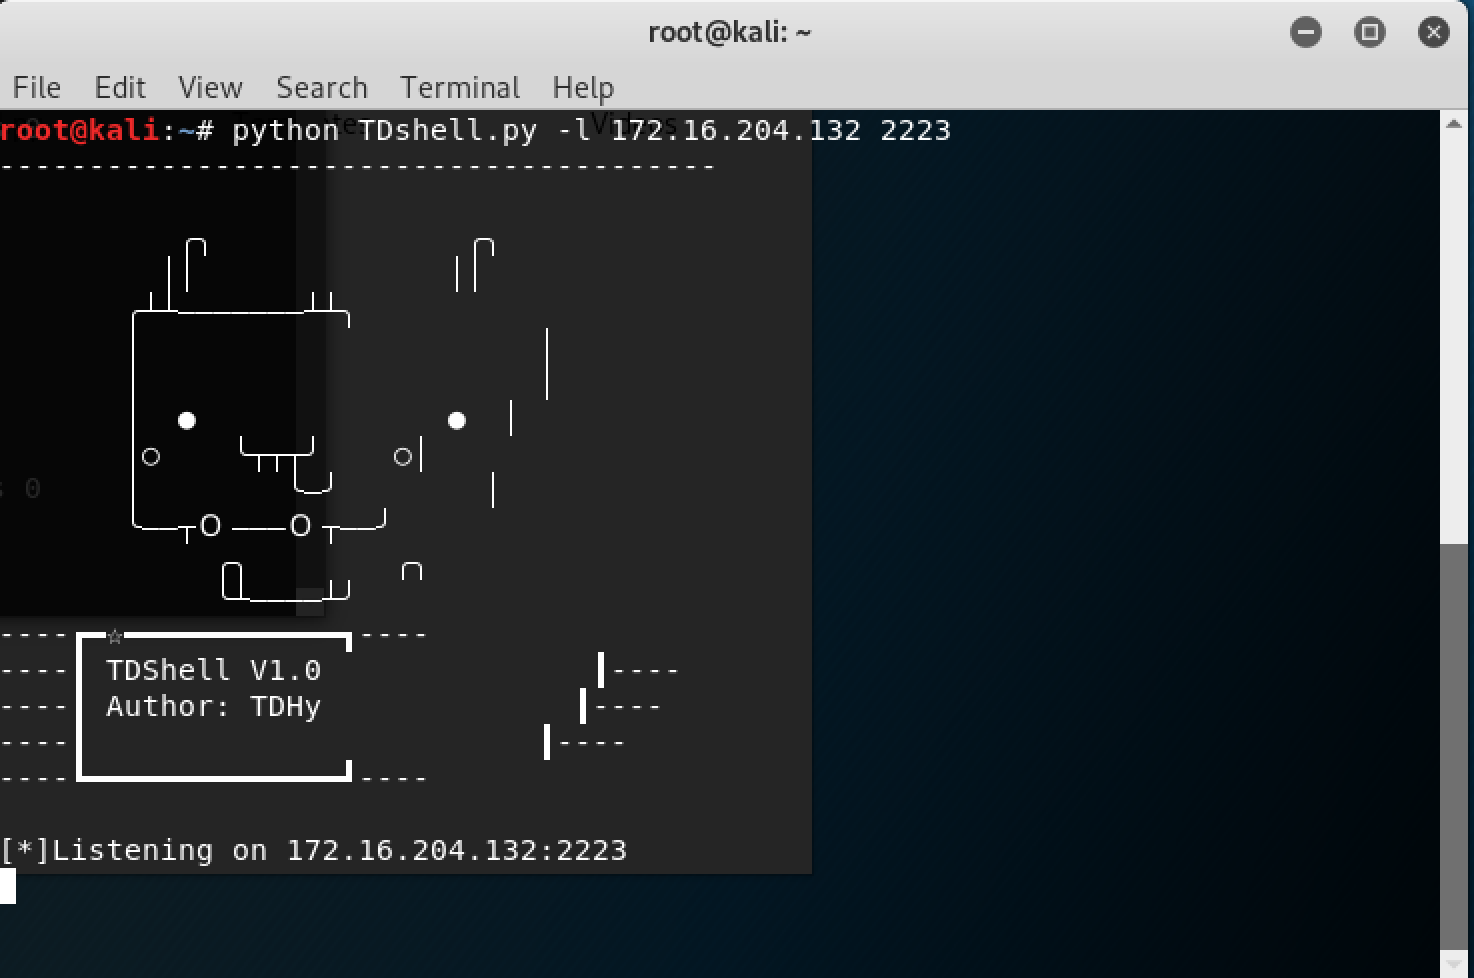
\includegraphics[scale=0.4]{Kali监听2223}
\caption{Kali监听2223端口}
\label{fig:3}
\end{figure}

Mac OS中在终端里通过切换命令跳转到木马程序当前路径下,或者在图形界面在木马程序文件夹上右击选中服务,选中在当前文件夹下以终端形式打开,再通过输入python TDshell.py -s [ip] [port]命令来启动攻击机主机客户端的监听功能,设定服务端IP地址和监听端口。
\begin{figure}[h]
\centering
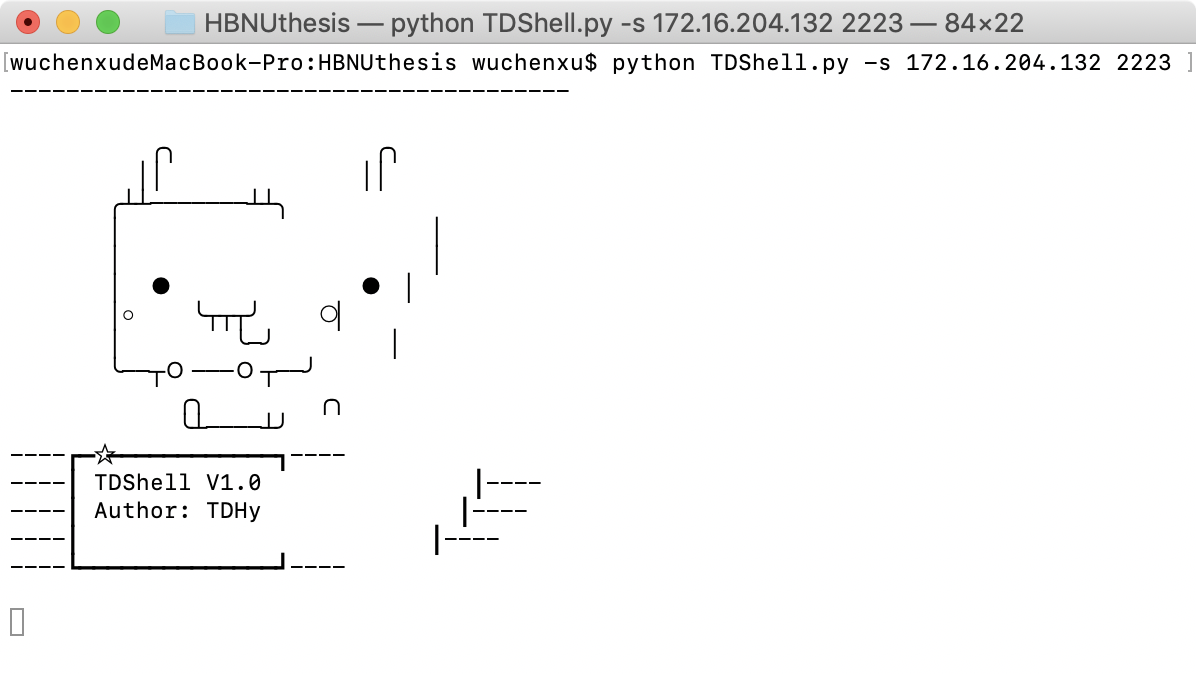
\includegraphics[scale=0.5]{macos反弹shell.png}
\caption{Mac OS 执行脚本客户端模式}
\label{fig:4}
\end{figure}


在上个步骤中,Mac OS 执行终端命令后,木马后门程序执行后,在宿主主机上发送一个看似正常的请求,请求通过socket发送到之前设定的ip地址和端口上,实现shell的反弹。这里就能够看到Kali的终端里已经可以执行宿主主机的命令。
\begin{figure}[h]
\centering
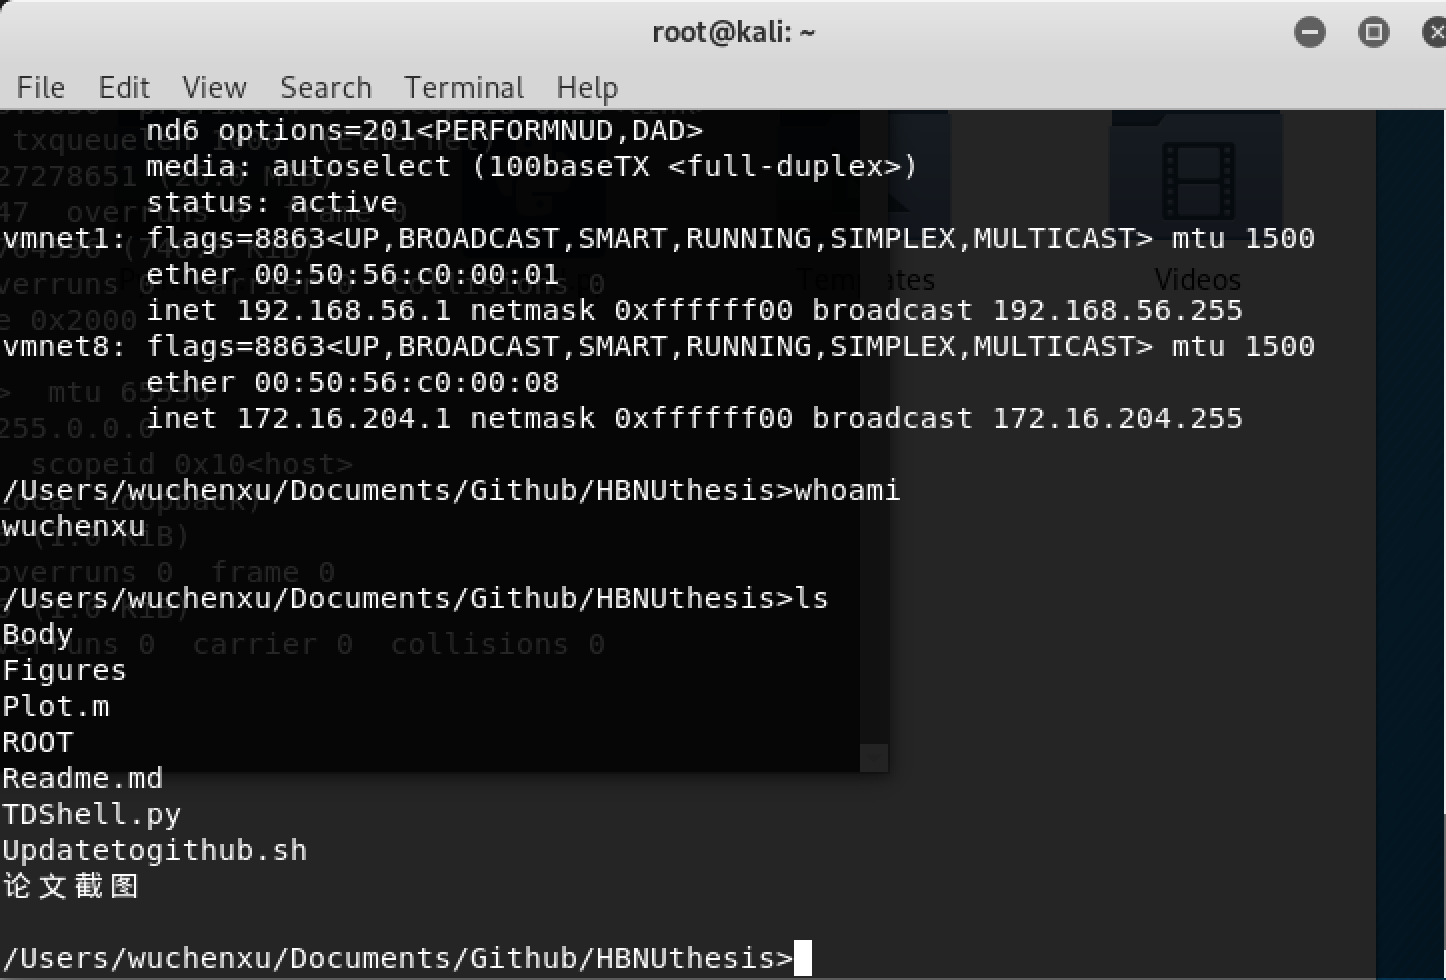
\includegraphics[scale=0.5]{kali拿到macosshell.png}
\caption{Kali拿到Mac OS shell}
\label{fig:5}
\end{figure}


\section{Linux环境下测试}
Ubuntu的不同版本情况不同,这里我们通过sudo apt-get install 命令安装python环境,同样Ubuntu中同样需要再次安装防火墙ufw,配置完成并启动后,攻击机主机开启脚本服务端模式开始监听,最后打开宿主主机上的脚本执行客户端命令,实现shell反弹。

\begin{itemize}
	\item 宿主主机:Ubuntu 18.04 
	\item 攻击主机:Kali Linux 2.0
\end{itemize}





先在Ubuntu中配置python环境。安装过程中需要等段一段时间,安装完成后可以通过终端如数python检测是否安装成功。
\begin{figure}[h]
\centering
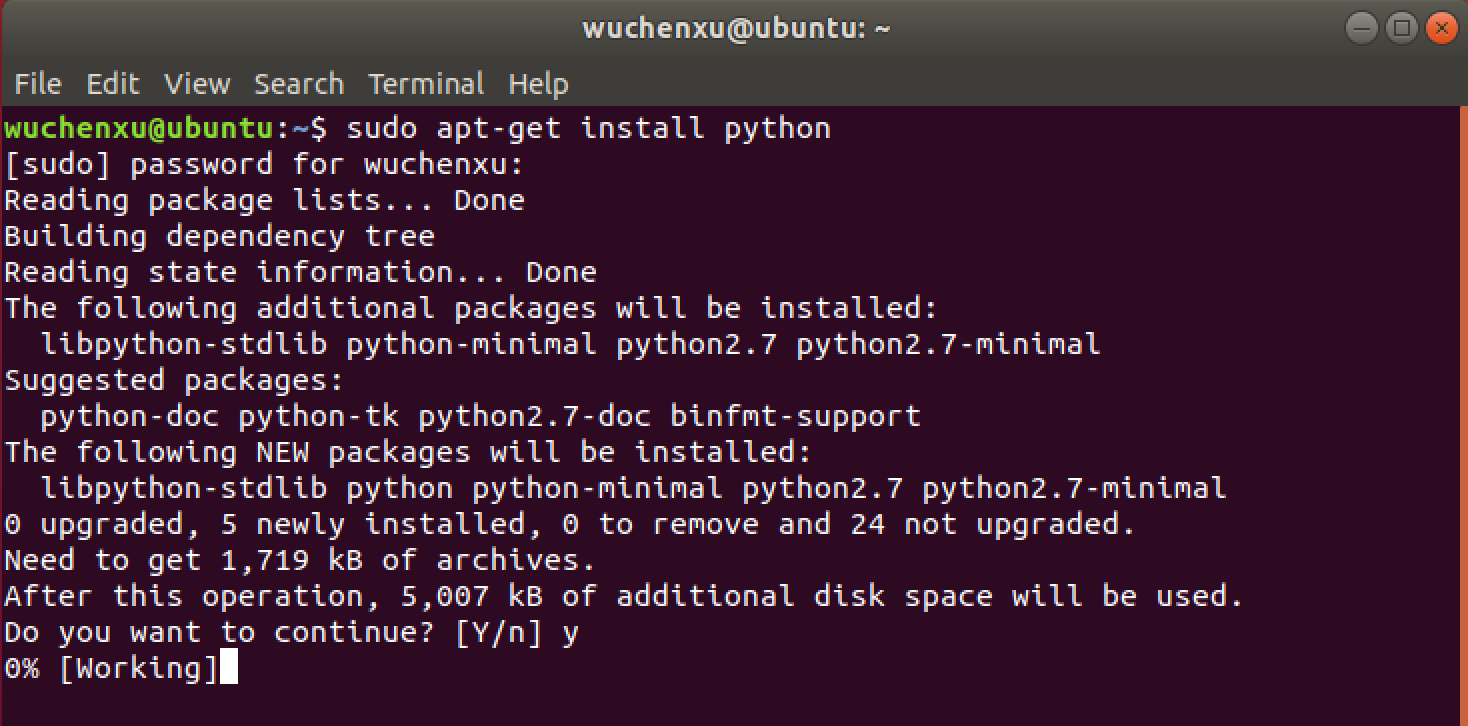
\includegraphics[scale=0.55]{Ubuntu安装python.png}
\caption{python环境配置}
\label{fig:6}
\end{figure}

Ubuntu通过sudo apt-get install ufw 安装防火墙,该防火墙属于Linux系统中较为典型的防火墙,通过第二章内容中的配置方法配置完成并打开。

\begin{figure}[h]
\centering
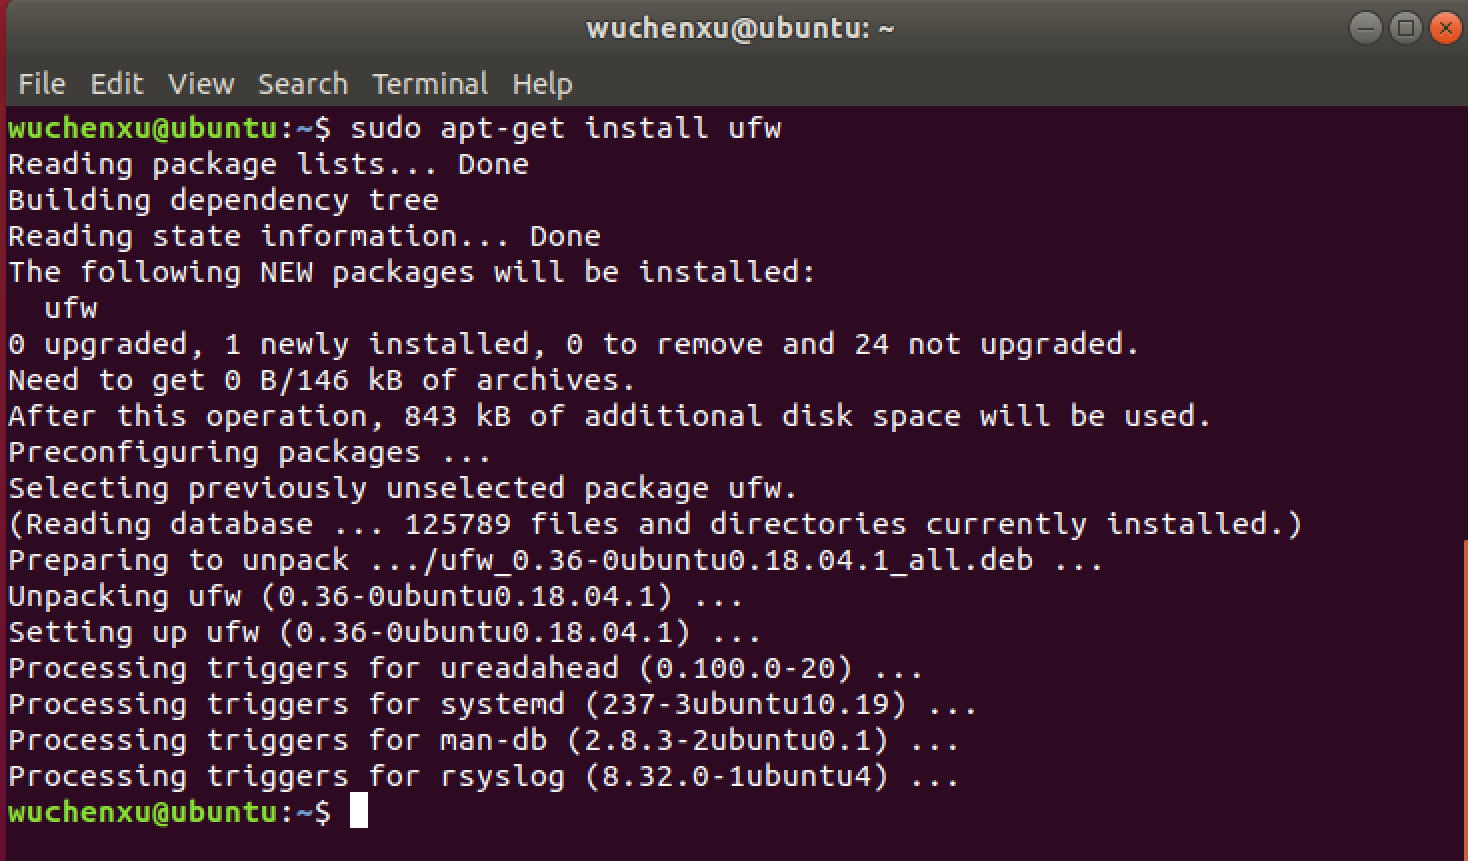
\includegraphics[scale=0.55]{ubuntu安装防火墙}
\caption{配置防火墙信息}
\label{fig:7}
\end{figure}

Kali Linux 2.0中在终端里通过切换命令跳转到木马程序当前路径下,或者在图形界面在木马程序文件夹内上右击,然后选中在当前文件夹下以终端形式打开,再通过输入python TDshell.py -l [ip] [port]命令来启动攻击机主机服务端的监听功能,设定服务端IP地址和监听端口。


\begin{figure}[h]
\centering
\includegraphics[scale=0.45]{Kali监听2222}
\caption{Kali监听2222端口}
\label{fig:3}
\end{figure}


Ubuntu中在终端里通过切换命令跳转到木马程序当前路径下,或者在图形界面在木马程序文件夹内选中在当前文件夹下以终端形式打开,再通过输入python TDshell.py -s [ip] [port]命令来启动攻击机主机客户端的监听功能,设定服务端IP地址和监听端口。


\begin{figure}[h]
\centering
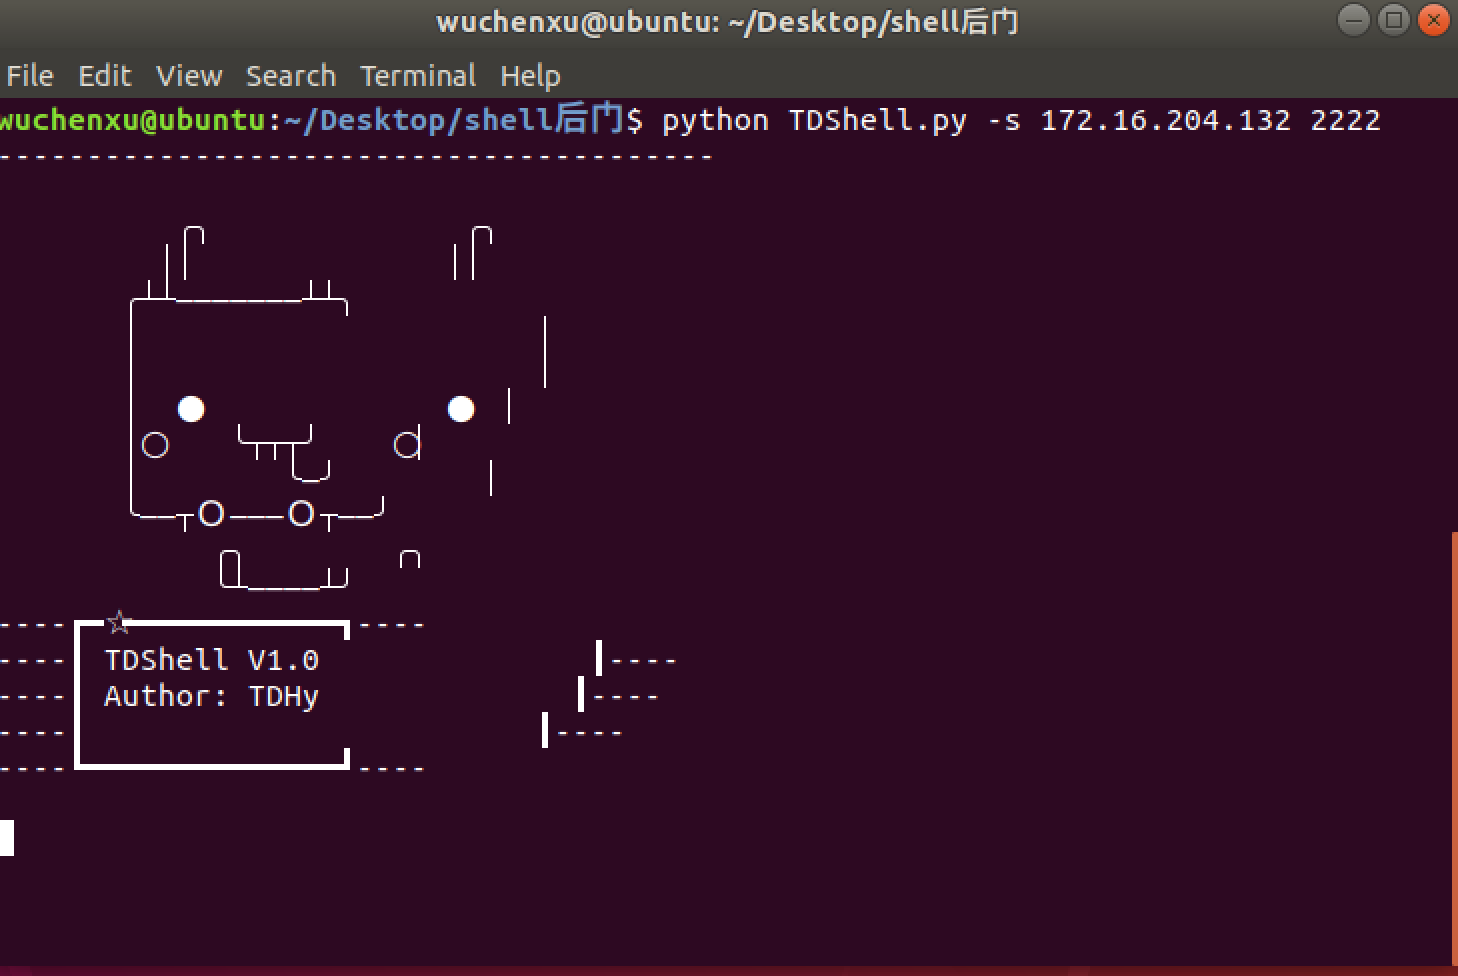
\includegraphics[scale=0.5]{ubuntu启动客户端.png}
\caption{Ubuntu执行脚本客户端模式}
\label{fig:4}
\end{figure}

切回Kali Linux之后可以看到终端中反弹到了宿主主机中当前文件夹的绝对路径,并且可以读写文件,执行终端命令。
\begin{figure}[h]
\centering
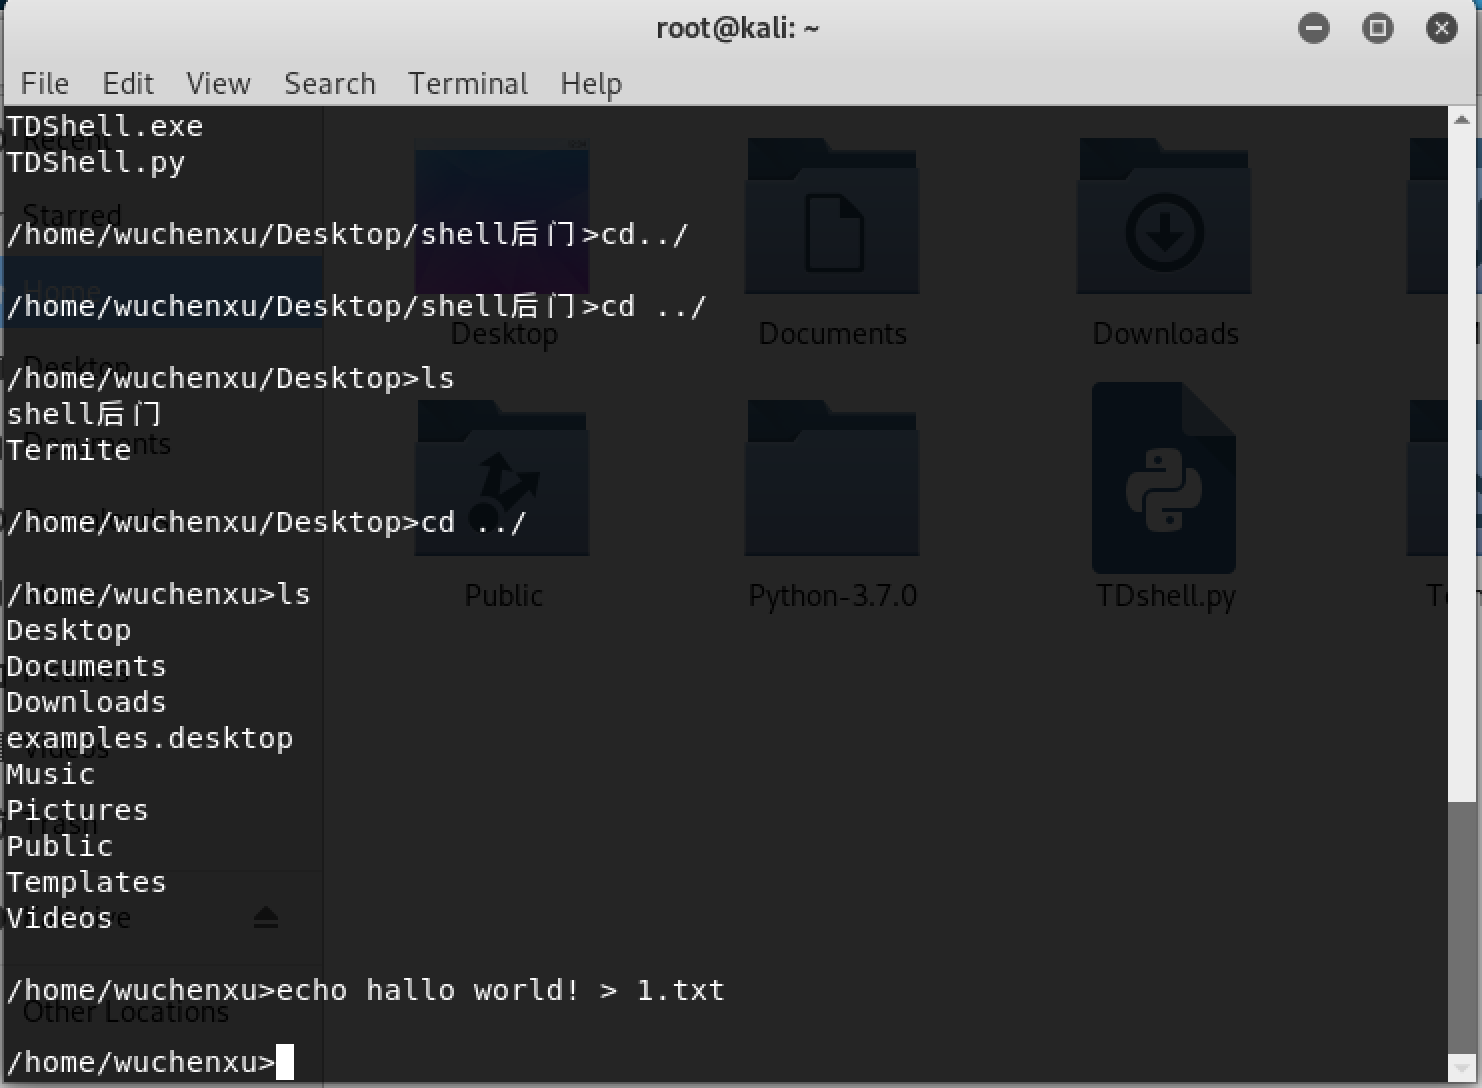
\includegraphics[scale=0.5]{kali确认ubuntu身份.png}
\caption{Kali拿到Ubuntu shell}
\label{fig:5}
\end{figure}






\section{Windows环境下测试}
\subsection{Windows 10环境测试}

\begin{itemize}
	\item 宿主主机:Windows 10 
	\item 攻击主机:Kali Linux 2.0
\end{itemize}




先在Windows 10中通过图形界面安装python安装包,勾选配置环境变量完成python环运行境的安装。
\begin{figure}[h]
\centering
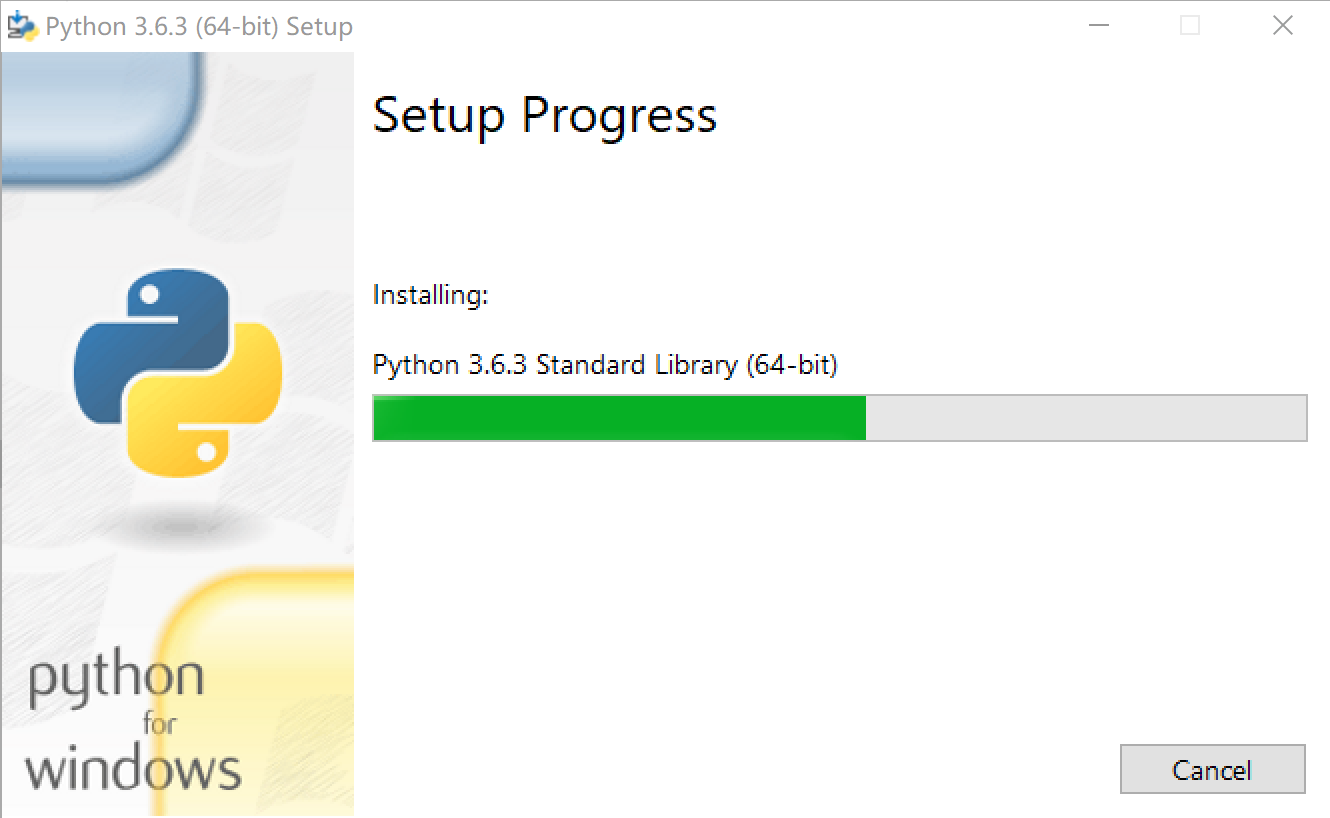
\includegraphics[scale=0.4]{win10安装python.png}
\caption{python环境配置}
\label{fig:6}
\end{figure}

因为Windows自身的原因,需要配置环境变量之后才可以在终端运行的时候通过命令行执行python程序。如图4-12 所示完成配置。
\begin{figure}[h]
\centering
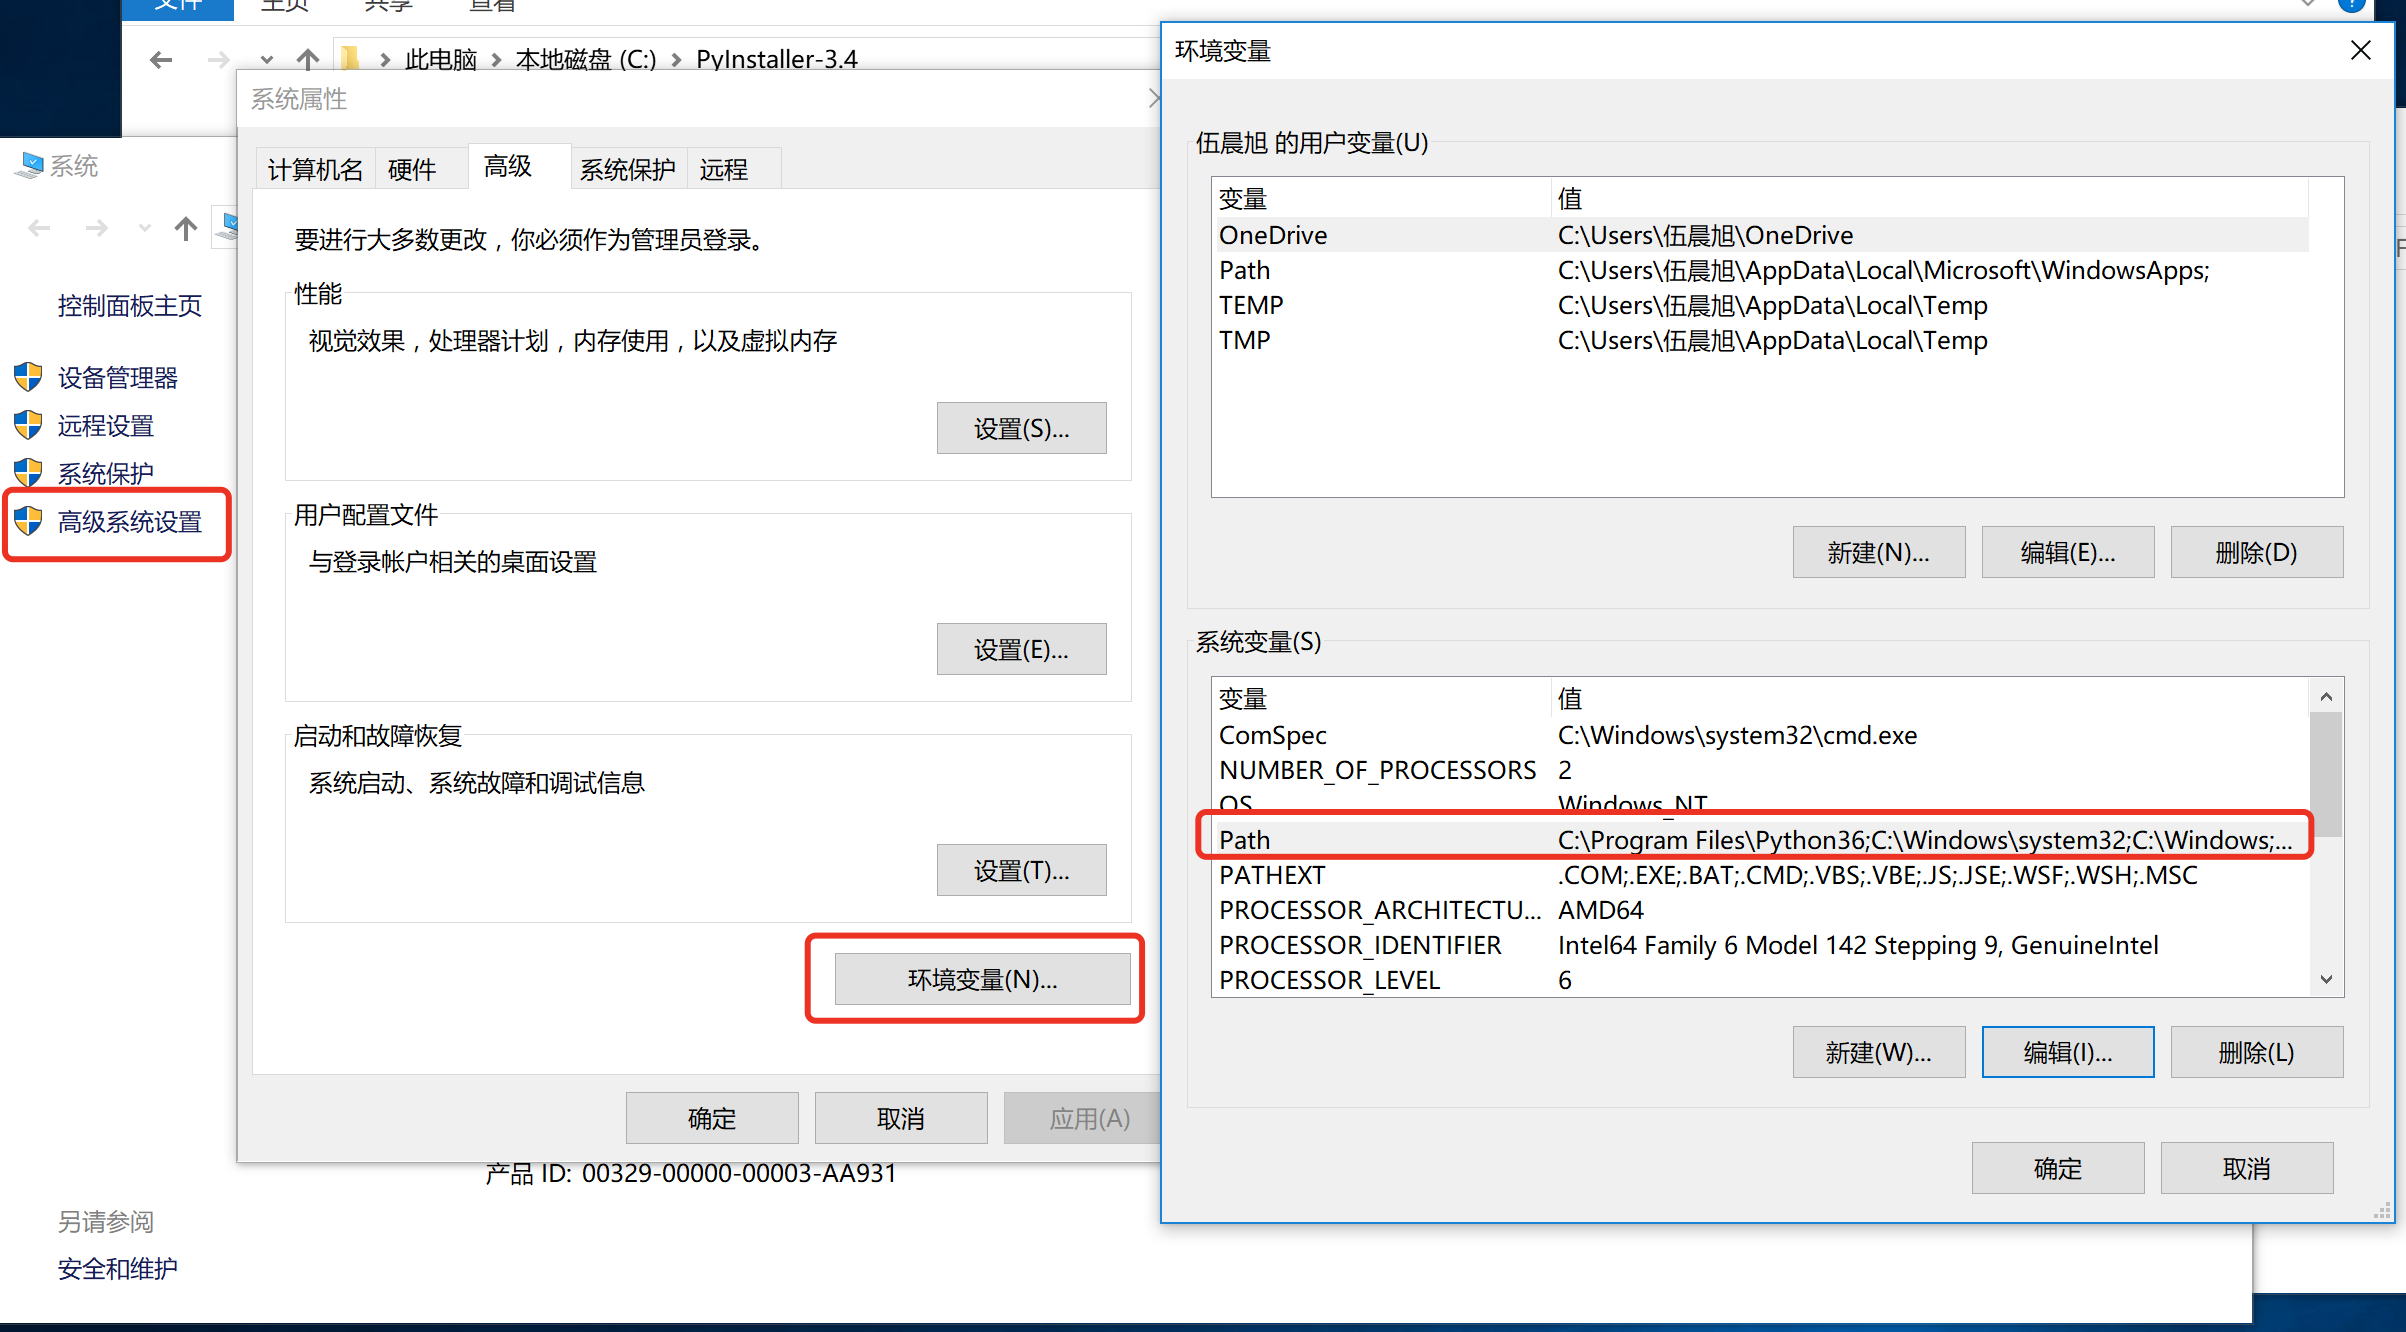
\includegraphics[scale=0.35]{win10设置环境变量.png}
\caption{python环境变量配置}
\label{fig:6}
\end{figure}


在宿主主机的控制面板中选择系统安全,进入防火墙设置。打开防火墙所有常规功能,Windows作为主流系统,该防火墙有一定的保护主机的功能。Windows配置防火墙信息。
\begin{figure}[h]
\centering
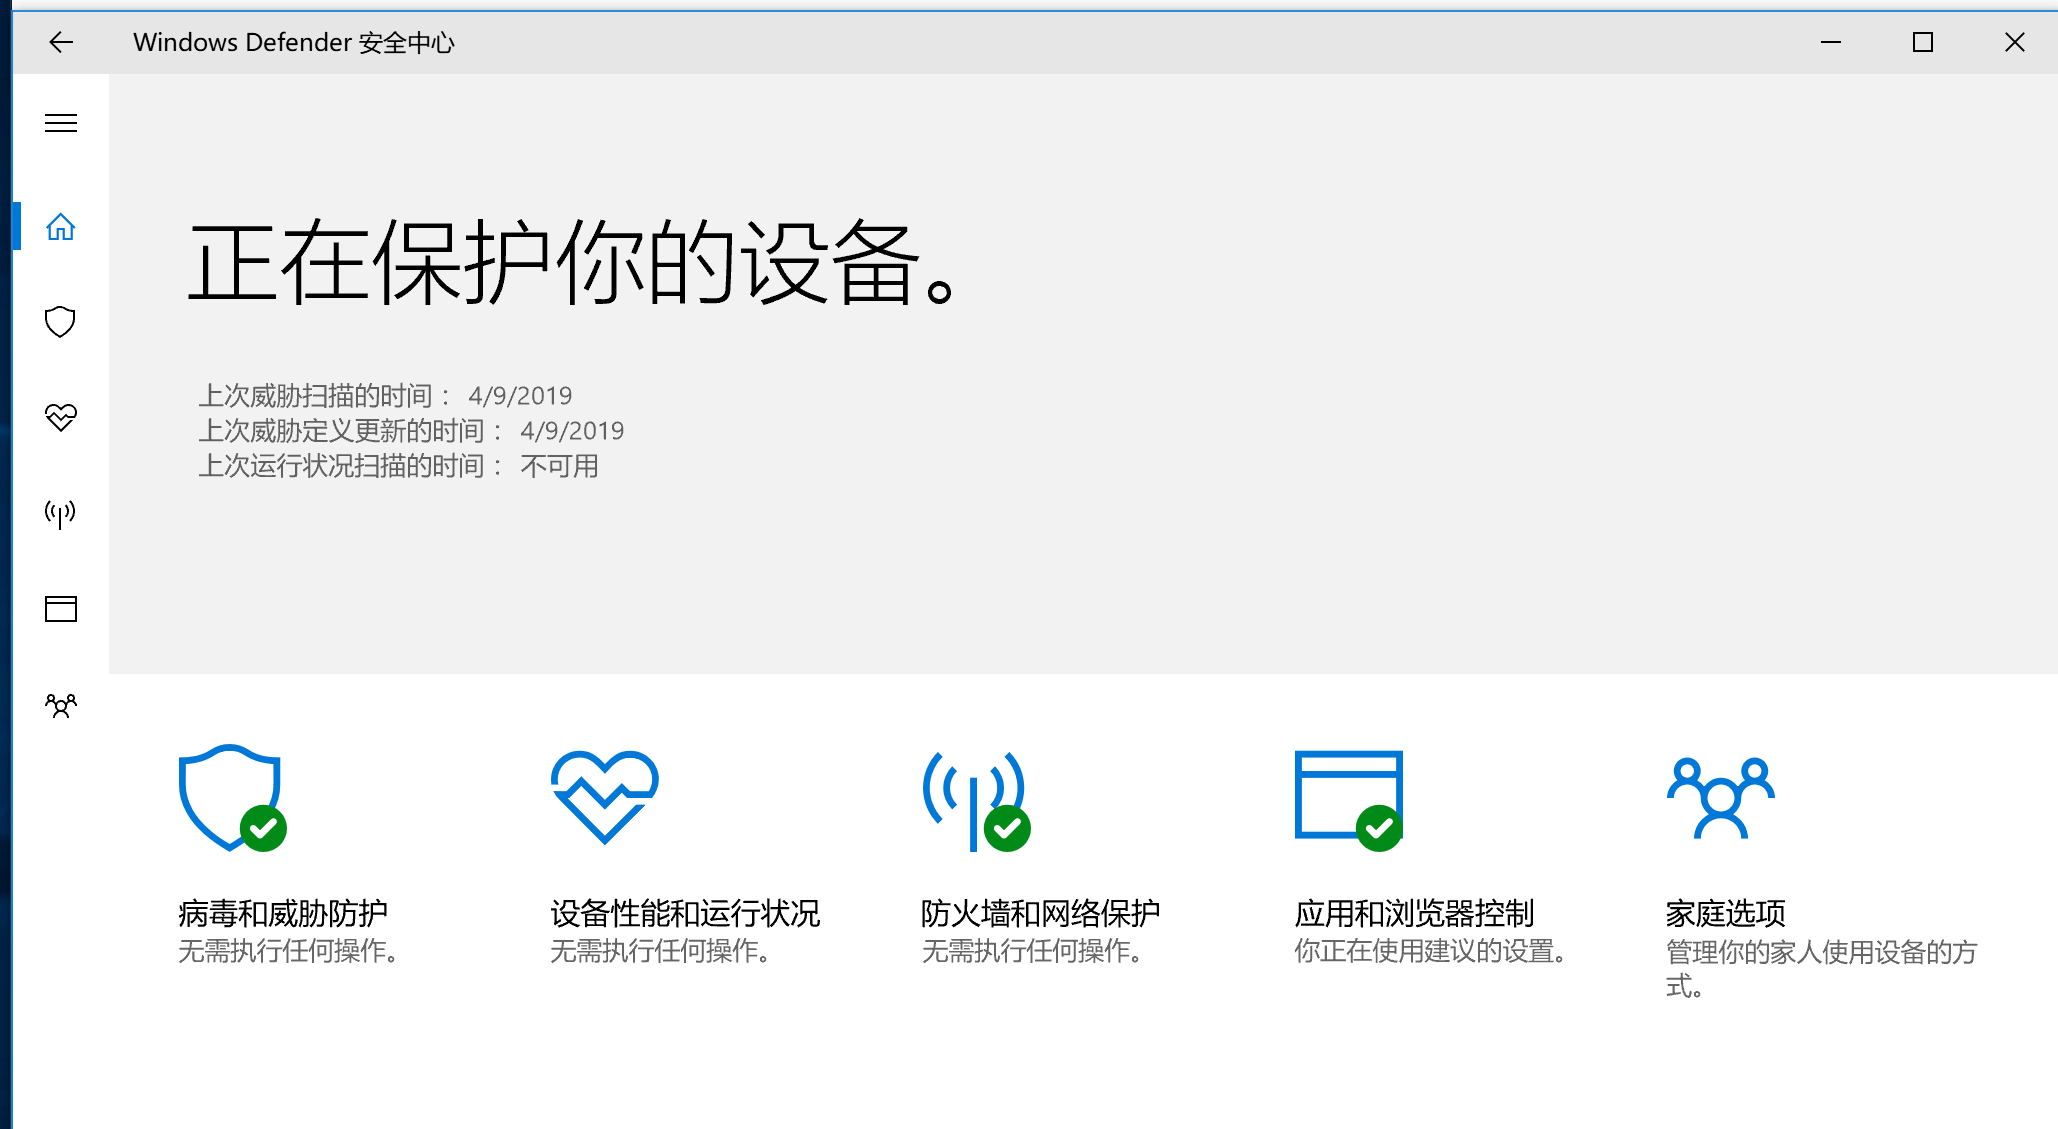
\includegraphics[scale=0.43]{win10打开防火墙.png}
\caption{配置防火墙信息}
\label{fig:7}
\end{figure}



Kali Linux 2.0中在终端里通过切换命令跳转到木马程序当前路径下,或者在图形界面在木马程序文件夹内上右击,然后选中在当前文件夹下以终端形式打开,再通过输入python TDshell.py -l [ip] [port]命令来启动攻击机主机服务端的监听功能,设定服务端IP地址和监听端口。

\begin{figure}[!h]
\centering
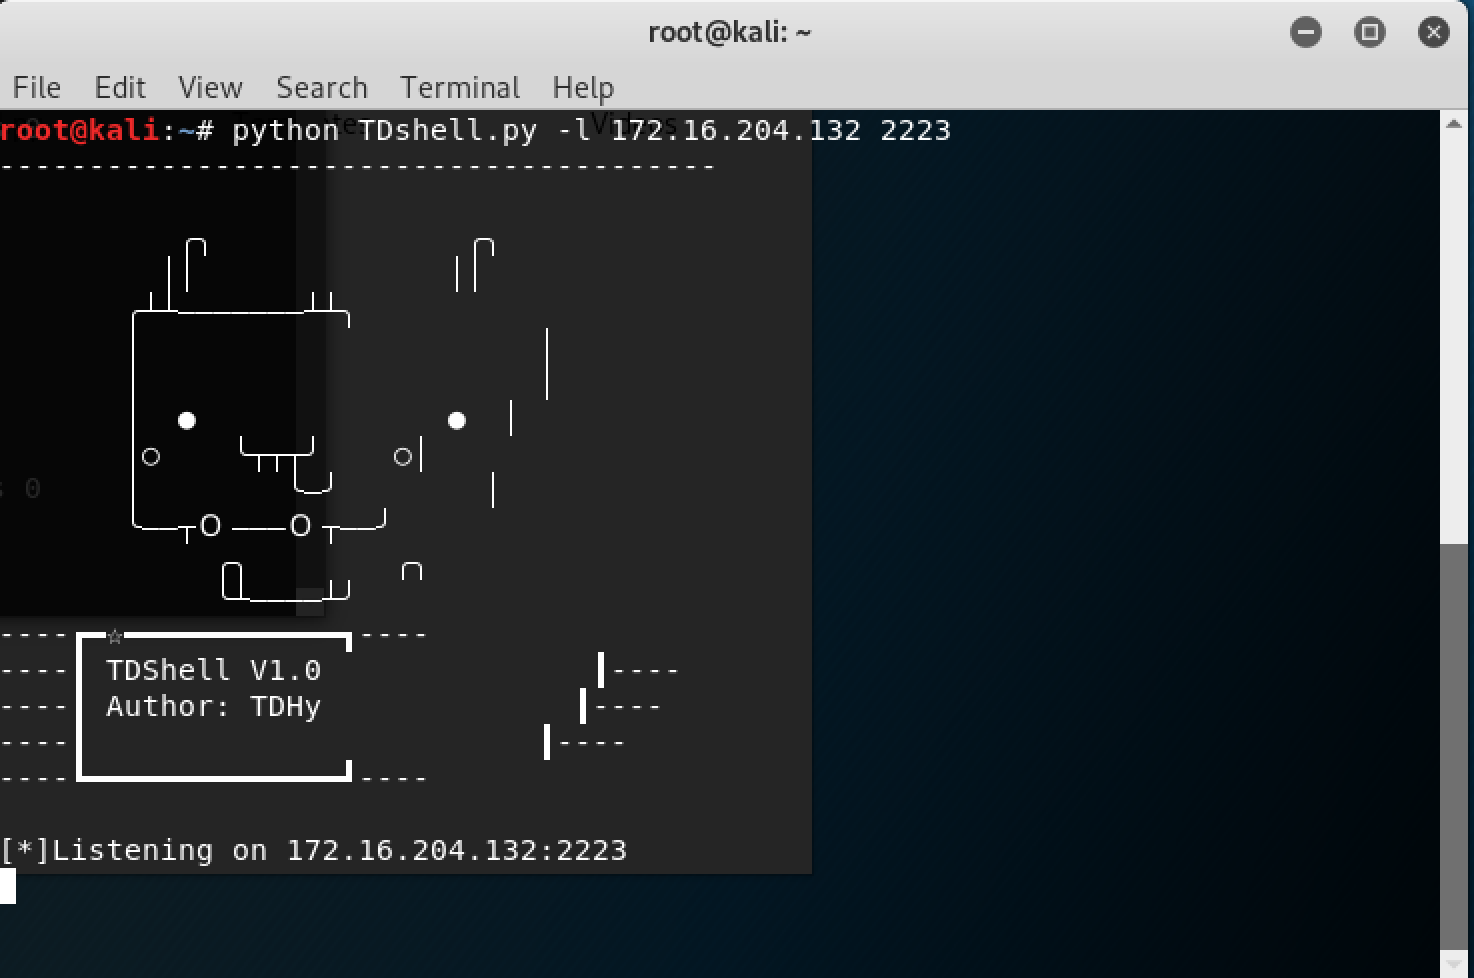
\includegraphics[scale=0.55]{Kali监听2223.png}
\caption{Kali监听2223端口}
\label{fig:3}
\end{figure}
在Windows端通过命令行窗口切换到木马后门程序所在的文件夹之后,通过设定的python环境变量,运行脚本文件,通过参数-s启用程序的客户端模式。

\begin{figure}[!h]
\centering
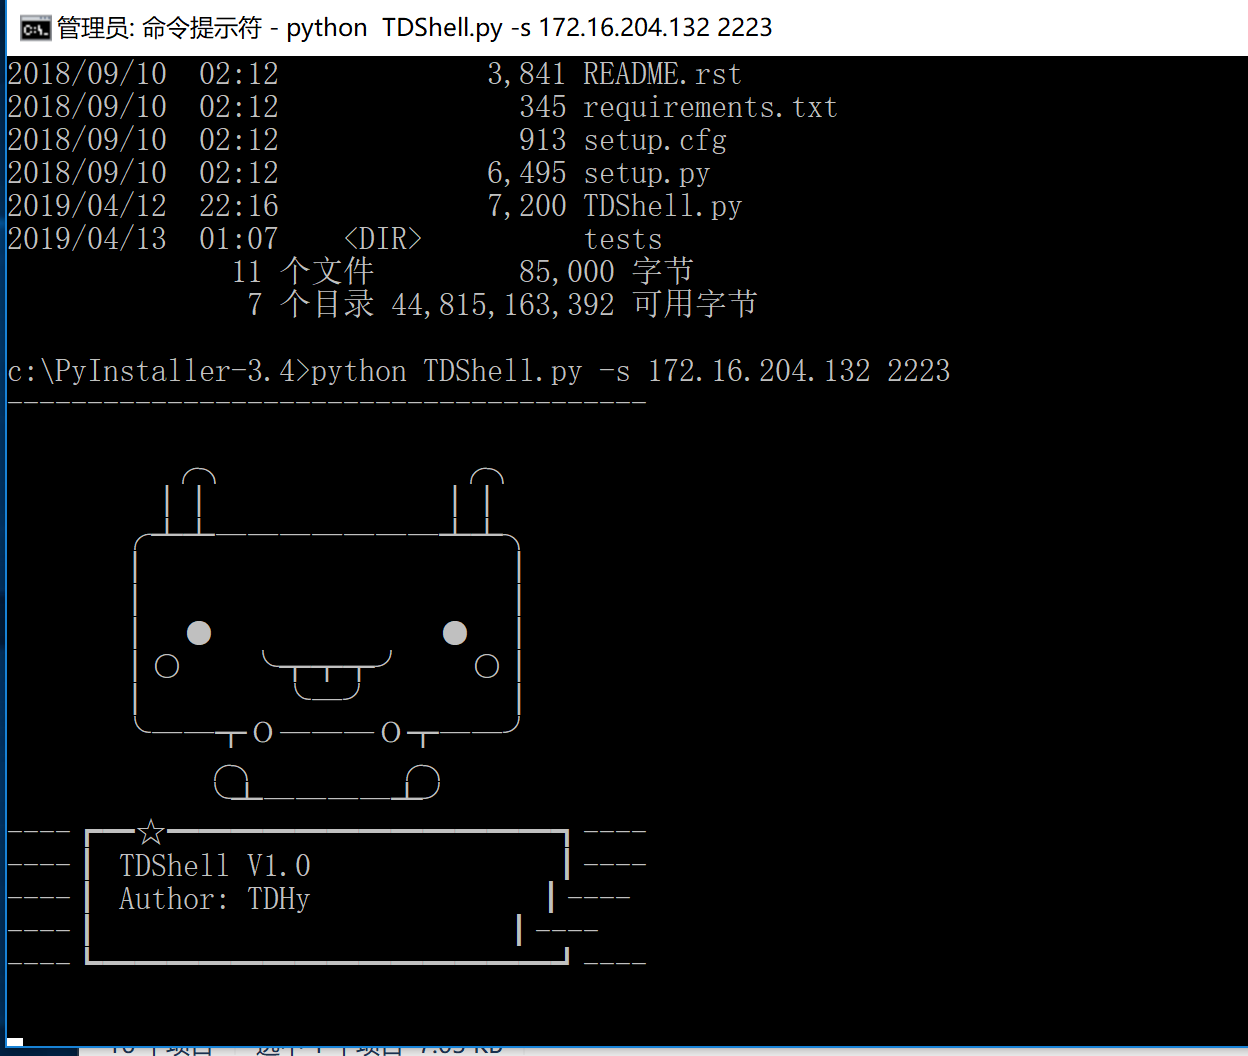
\includegraphics[scale=0.6]{win10启动客户端.png}
\caption{Windows 10执行脚本客户端模式}
\label{fig:4}
\end{figure}

\begin{figure}[!h]
\centering
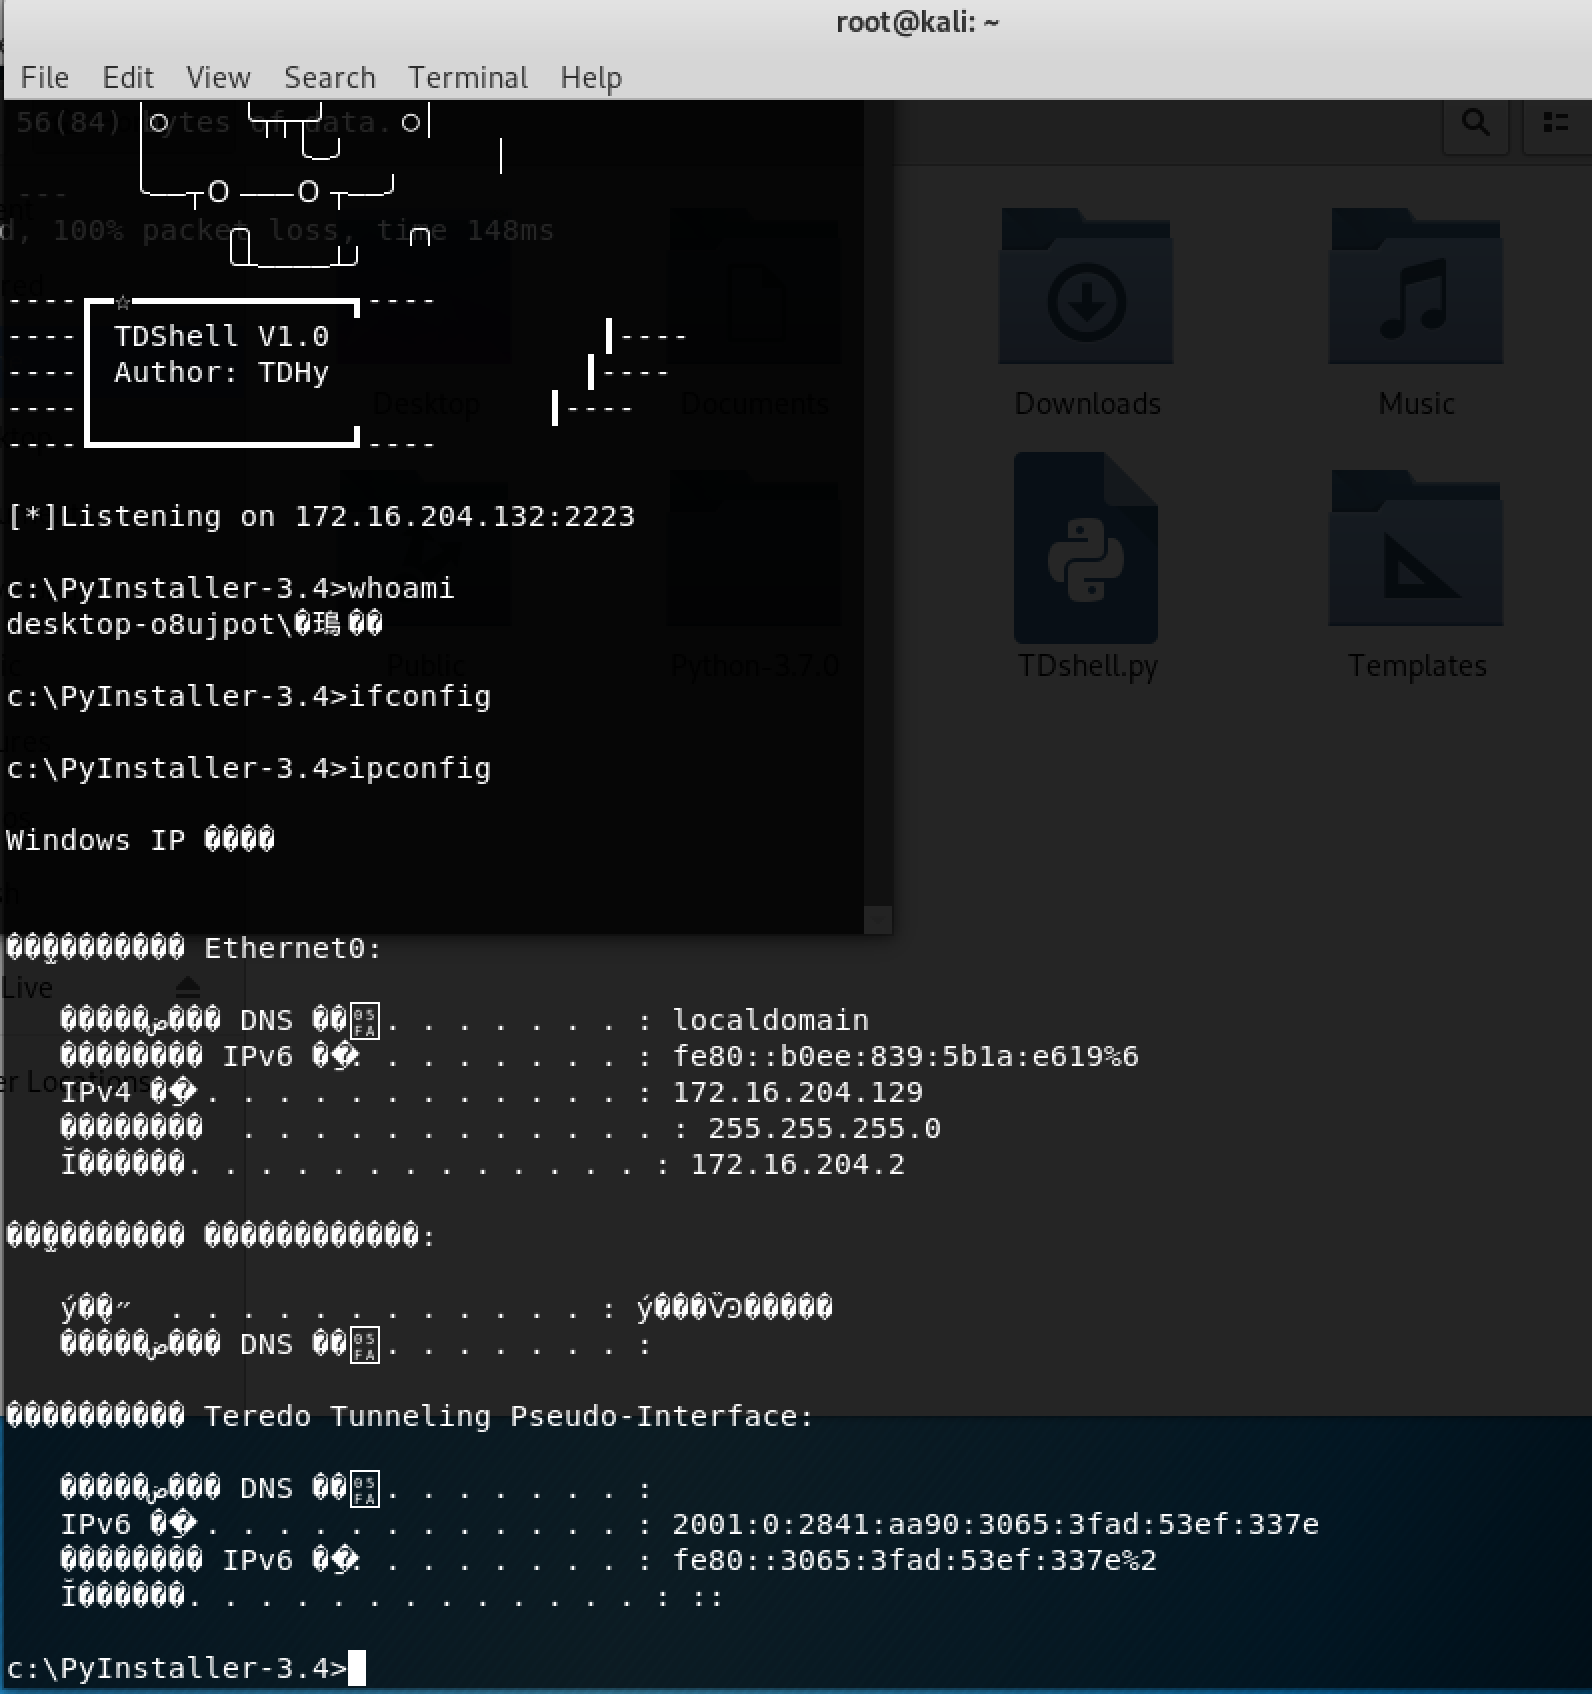
\includegraphics[scale=0.5]{kali确认win10身份.png}
\caption{Kali拿到Windows 10 shell}
\label{fig:5}
\end{figure}

随后看到在Kali Linux端收到来自Windows 10反弹过来的shell,可以执行恶意代码。




\subsection{Windows Server 2012 R2环境测试}
Windows Server 作为微软公司面向企业开发的服务器操作系统有着很高的安全指数,同时具备着最严格的账户管理规则,所以我们在测试环节中加入了Windows Server的测试环节,该系统的部分操作和WIndows 10相似,所以我们会跳过部分内容,简述测试过程。


\begin{itemize}
	\item 宿主主机:Windows server 2012 R2
	\item 攻击主机:Kali Linux 2.0
\end{itemize}



在Windows server 2012 R2 中配置python环境和在Windows 10中配置的情况是一样的,所以这里不再赘述。


同样我们首先要配置Windows server R12防火墙信息。在控制面板中选择系统与安全,进入防火墙设置窗口,选择启用防火墙之后点击确认键。\\

\begin{figure}[h]
\centering
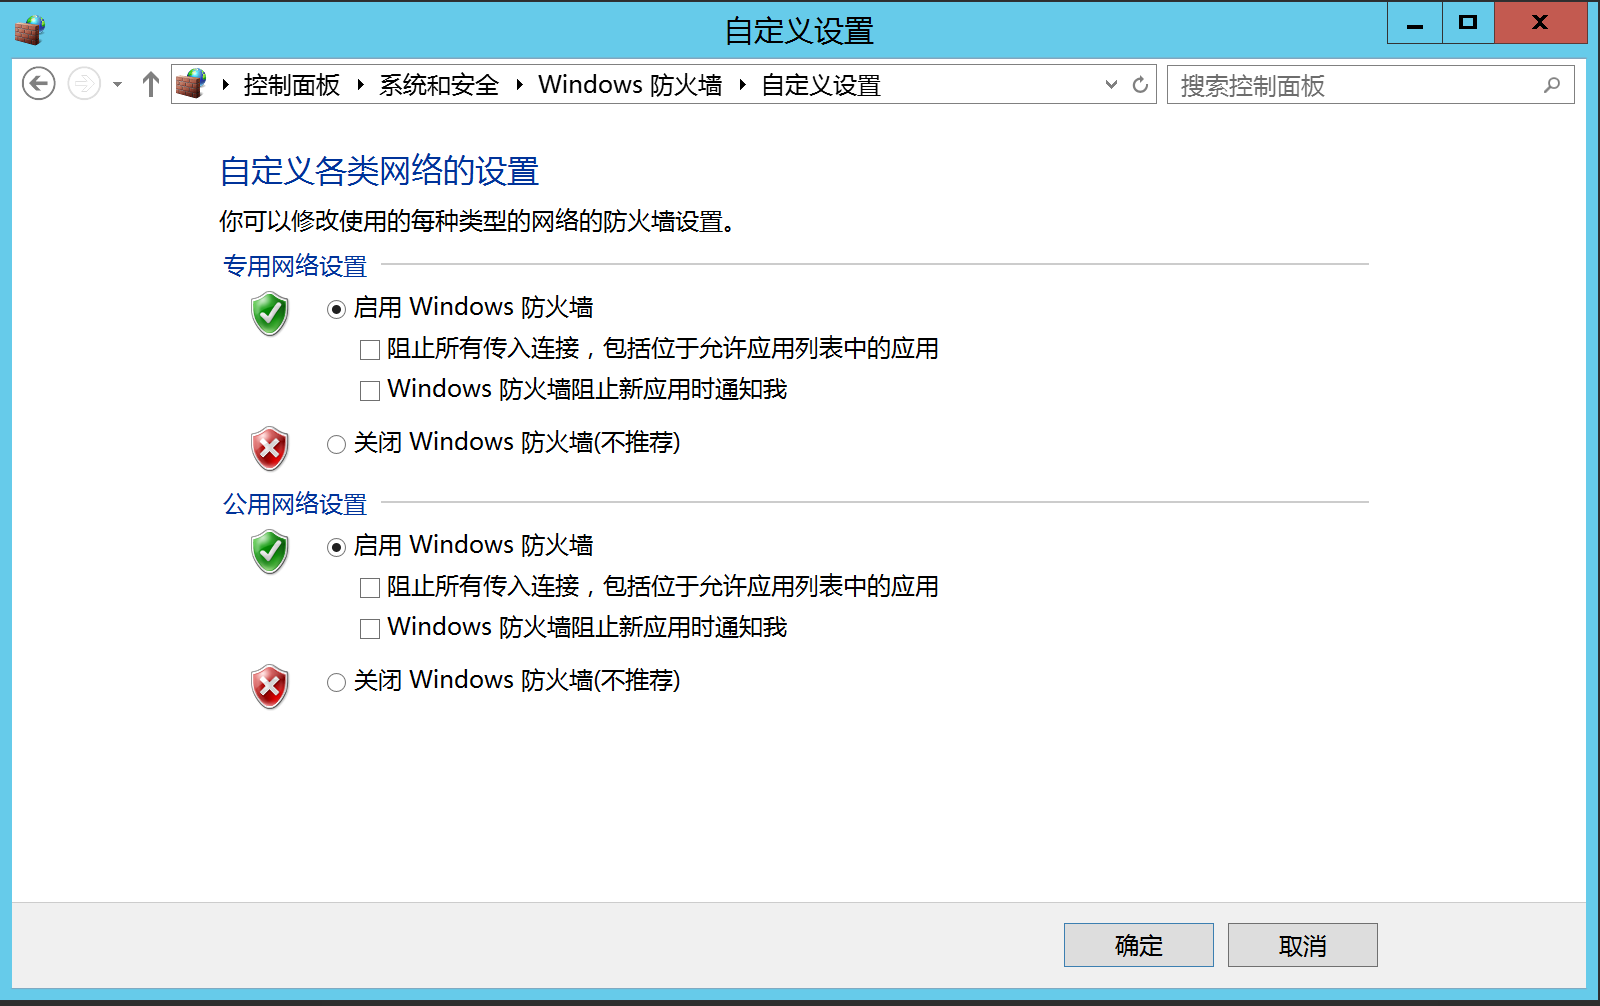
\includegraphics[scale=0.4]{winser打开防火墙.png}
\caption{配置防火墙信息}
\label{fig:7}
\end{figure}



Kali Linux 2.0中在终端里通过切换命令跳转到木马程序当前路径下,或者在图形界面在木马程序文件夹内上右击,然后选中在当前文件夹下以终端形式打开,再通过输入python TDshell.py -l [ip] [port]命令来启动攻击机主机服务端的监听功能,设定服务端IP地址和监听端口。
\begin{figure}[!h]
\centering
\includegraphics[scale=0.62]{Kali监听2224}
\caption{Kali监听2224端口}
\label{fig:3}
\end{figure}



在Windows Server 2012 R2中,我们选择使用管理员权限打开cmd之后,敲入之前安装配置过的python环境变量,运行后门程序,通过参数-s设定客户端模式,同时设置好服务器端的ip和端口。
\begin{figure}[!h]
\centering
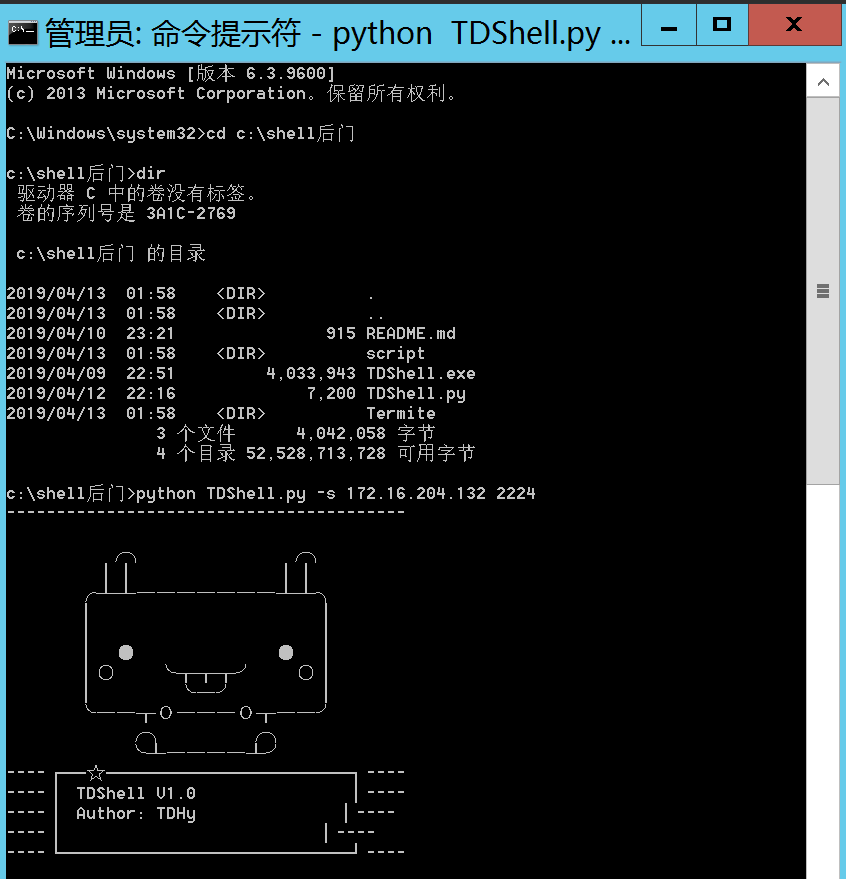
\includegraphics[scale=0.55]{winser启动客户端.png}
\caption{Windows server 2012 R2 执行脚本客户端模式}
\label{fig:4}
\end{figure}




最后我们在Kali Linux的监听界面上可以看到来自Windows Server 2012 R2反弹回来的shell,通过whoami命令和ipconfig来确定受害者主机信息确认测试成功。
\begin{figure}[!h]
\centering
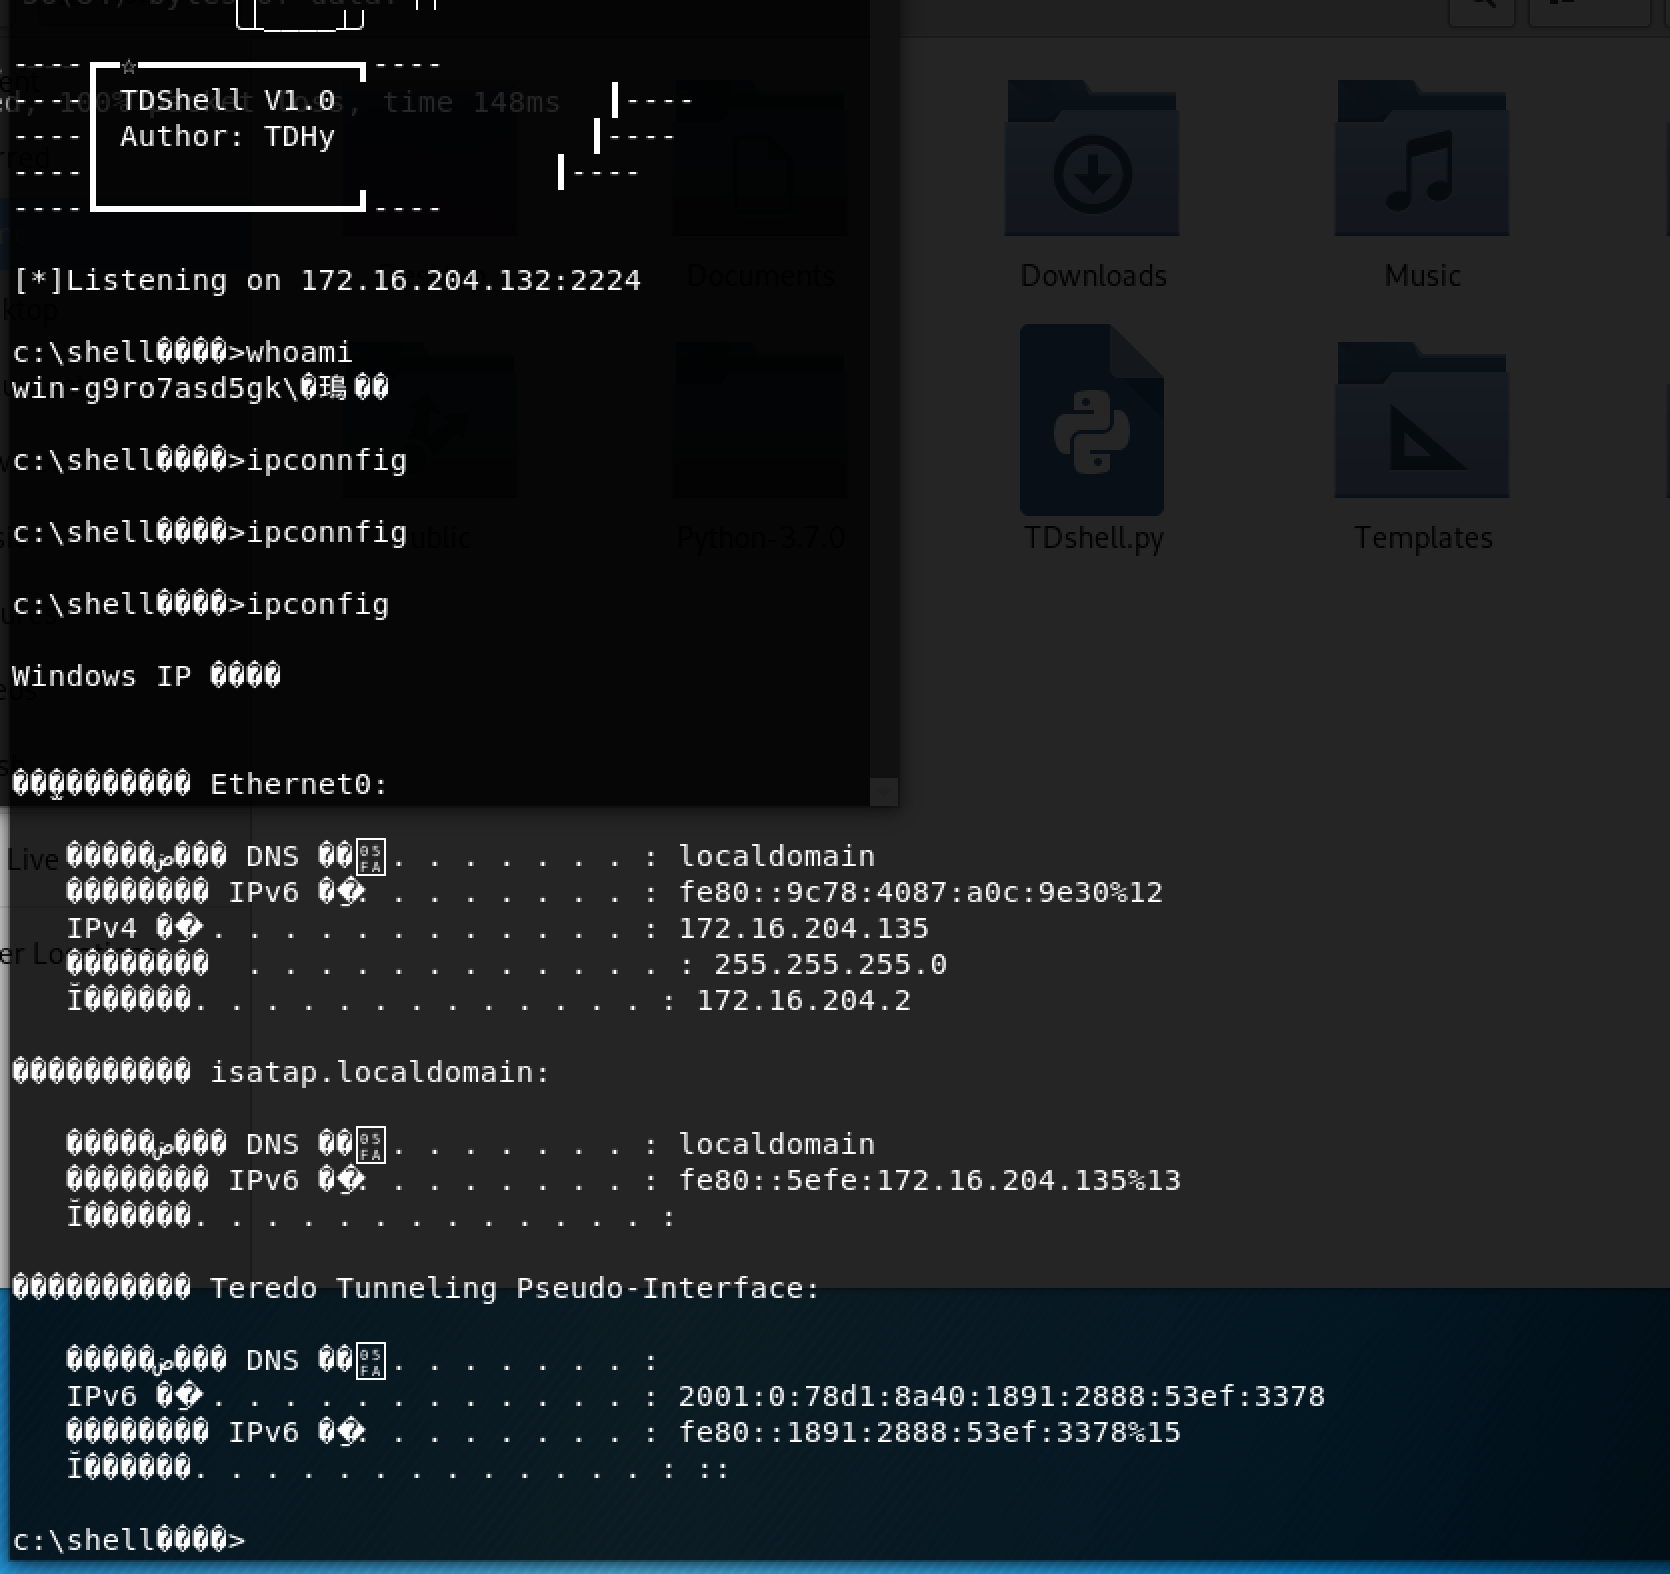
\includegraphics[scale=0.35]{kali拿到winsershell.png}
\caption{Kali拿到Windows server 2012 R2 shell}
\label{fig:5}
\end{figure}



